\documentclass[12pt, a4paper]{article}
\usepackage[margin=1in]{geometry}
\usepackage{../auxiliary/utilities/preamble}

\newcommand{\titulo}{Tarea 3: Transformadas de Laplace}
\newcommand{\fecha}{11 de febrero de 2024}

\begin{document}
\sffamily
\begin{titlepage}
    \begin{center}
        
\includegraphics[width=0.15\textwidth]{../auxiliary/assets/unam.png}
        \hspace{0.6\textwidth}
        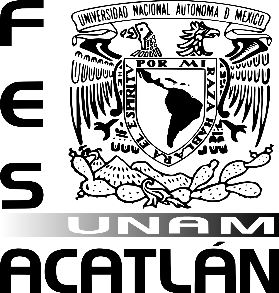
\includegraphics[width=0.15\textwidth]{../auxiliary/assets/fes.png}

        \vspace*{5cm}
        \LARGE
        \textbf{\titulo}

        \vspace{1cm}
        \large
        Camargo Badillo Luis Mauricio \\
        \vspace{1.5cm}
        \textit{\fecha}

        \vfill

        \vspace{0.5cm}
        Ecuaciones Diferenciales II \\
        Oscar Gabriel Caballero Martínez \\
        Grupo 2602 \\
        \textbf{Matemáticas Aplicadas y Computación}\\
    \end{center}
\end{titlepage}


\tableofcontents
\newpage

\setcounter{section}{1}
\section{\texorpdfstring{\(f(t) = c\)}{f (t) = c}}

Calculamos la transformada de Laplace de \(f(t) = c\):
\begin{align*}
    \mathcal{L}\{c\}&=\int_0^{\infty}e^{-st}(c)\\
    &=\int_0^{\infty}ce^{-st}\\
    &=c\int_0^{\infty}e^{-st}\\
    &=\lim_{b\to\infty}c\int_0^b e^{-st}\ dt
\end{align*}
Sustiuimos con \(u=-st \implies du =-s\ dt\), obteniendo:
\begin{align*}
	&=\lim_{b\to\infty}-\frac{c}{s}\left[\int_0^{-sb}  e^u\ du\right] \\
	&=-\frac{c}{s}\lim_{b\to\infty}\left[e^u\big|_0^{-sb}  \right]\\
	&=-\frac{c}{s}\lim_{b\to\infty}\left[e^{-sb}-e^{0}\right]\\
	&=-\frac{c}{s} \left[ \lim_{b\to\infty} e^{-sb} - 1 \right]
\end{align*}
Cuando \(s > 0 \implies -s < 0\), por lo que podemos escribir:
\begin{align*}
	&= -\frac{c}{s} \left[ \lim_{b\to-\infty} e^{b} - 1 \right] \\
	&= -\frac{c}{s} \left[ 0 - 1 \right] \\
	&= \frac{c}{s}
\end{align*}
Así, finalmente:
\[
\mathcal{L}\{c\}=\frac{c}{s} \qquad s > 0
\]

\setcounter{section}{4}
\section{\texorpdfstring{\(f(t) = t^3\)}{f (t) = t 3}}

Calculamos la transformada de Laplace de \(f(t) = t^{3}\):
\begin{align} \label{eq:primera-exp}
    \mathcal{L}\{t^3\}&=\int_0^\infty e^{-st}t^3\ dt\ \notag \\
    &=\lim_{b\to\infty}\int_0^b e^{-st}t^3\ dt
\end{align}
Enfoquémonos en la integral en sí. Para resolverla, integramos por partes, utilizando \(u= t^3 \implies du= 3t^2\ dt\) y \(dv=e^{-st}\ dt \implies v=-\frac{1}{s}e^{-st}\):
\begin{align} \label{eq:primera-int}
    \int_0^b e^{-st}t^3\ dt &= \left. \left( -\frac{t^3 e^{-st}}{s}\right) \right|_0^b + \frac{3}{s} \int_0^b e^{-st}t^2 \ dt \notag \\
    &= \left( -\frac{b^3e^{-sb}}{s}+\frac{0}{s} \right) +\frac{3}{s}\int_0^b e^{-st}t^2\ dt \notag \\
    &=-\frac{b^3e^{-sb}}{s} + \frac{3}{s}\int_0^b e^{-st}t^2\ dt
\end{align}
Observemos que tenemos otra integral. Resolvámosla también por partes, utilizando \(u=t^2\implies du=2t\ dt\) y \(dv=e^{-st}dt\implies v=-\frac{1}{s}e^{-st}\):
\begin{align} \label{eq:segunda-int}
    \int_0^b e^{-st}t^2\ dt&= \left. \left( -\frac{t^2 e^{-st}}{s} \right) \right|_0^b + \frac{2}{s} \int_0^b e^{-st}t\ dt \notag \\
    &= \left( -\frac{b^2e^{-sb}}{s}+\frac{0}{s} \right) + \frac{2}{s} \int_0^b e^{-st}t \ dt \notag \\
    &=-\frac{b^2e^{-sb}}{s}+\frac{2}{s}\int_0^b e^{-st}t \ dt \notag \\
    &=-\frac{b^2e^{-sb}}{s}+\frac{2}{s}\int_0^b e^{-st}t \ dt
\end{align}
Una vez más, tenemos otra integral. Otra vez resolvamos por partes utilizando \(u=t\implies du=dt\) y \(dv=e^{-st}\ dt\implies v=-\frac{1}{s}e^{-st}\), obteniendo:
\begin{align} \label{eq:tercera-int}
    \int_0^b e^{-st}t\ dt &= \left. \left(-\frac{te^{-st}}{s} \right) \right|_0^b + \frac{1}{s} \int_0^b e^{-st}\ dt \notag \\
    &= \left( -\frac{be^{-sb}}{s}+\frac{0}{s} \right) +\frac{1}{s} \int_0^b e^{-st}\ dt \notag \\
    &=-\frac{be^{-sb}}{s}+\frac{1}{s}\int_0^b e^{-st}\ dt
\end{align}
Tenemos una última integral, pero esta vez la resolveremos con una sustitución \(u = -st \implies du = -s\ dt\), obteniendo:
\begin{align} \label{eq:cuarta-int}
    \int_0^b e^{-st}\ dt&=-\frac{1}{s}\int_0^{-sb} e^u\ du \notag \\
    &=-\frac{1}{s} \left. \left( e^u \right) \right|_0^{-sb} \notag \\
    &=-\frac{e^{-sb}}{s}+\frac{e^{-s(0)}}{s} \notag \\
    &=-\frac{e^{-sb}}{s}+\frac{1}{s}
\end{align}
Sustituyendo todas estas expresiones donde corresponden, obtenemos:
\begin{align*}
    \mathcal{L}\{t^3\} &= \lim_{b\to\infty}\int_0^b e^{-st}t^3\ dt & (\ref{eq:primera-exp}) \\
	&=\lim_{b\to\infty} \left[ -\frac{b^3e^{-sb}}{s}+\frac{3}{s}\int_0^b e^{-st}t^2\ dt \right] & \text{sust. } (\ref{eq:primera-int}) \\
    &=\lim_{b\to\infty} \left[ -\frac{b^3e^{-sb}}{s}+\frac{3}{s}\left(-\frac{b^2e^{-sb}}{s}+\frac{2}{s}\int_0^b e^{-st}t\ dt\right) \right] & \text{sust. } (\ref{eq:segunda-int}) \\
    &=\lim_{b\to\infty} \left[ -\frac{b^3e^{-sb}}{s}+\frac{3}{s}\left(-\frac{b^2e^{-sb}}{s}+\frac{2}{s}\left[-\frac{be^{-sb}}{s}+\frac{1}{s}\int_0^b e^{-st}dt\right]\right) \right] & \text{sust. } (\ref{eq:tercera-int}) \\
    &=\lim_{b\to\infty} \left[ -\frac{b^3e^{-sb}}{s}+\frac{3}{s}\left(-\frac{b^2e^{-sb}}{s}+\frac{2}{s}\left[-\frac{be^{-sb}}{s}+\frac{1}{s}\left(-\frac{e^{-sb}}{s}+\frac{1}{s}\right)\right]\right) \right] & \text{sust. } (\ref{eq:cuarta-int}) \\
    &=\lim_{b\to\infty} \left[ -\frac{b^3e^{-sb}}{s}+\frac{3}{s}\left(-\frac{b^2e^{-sb}}{s}+\frac{2}{s}\left[-\frac{be^{-sb}}{s}-\frac{e^{-sb}}{s^2}+\frac{1}{s^2}\right]\right) \right] \\
    &=\lim_{b\to\infty} \left[ -\frac{b^3e^{-sb}}{s}+\frac{3}{s}\left(-\frac{b^2e^{-sb}}{s}-\frac{2be^{-sb}}{s^2}-\frac{2e^{-sb}}{s^3}+\frac{2}{s^3}\right) \right] \\
    &=\lim_{b\to\infty} \left[ -\frac{b^3e^{-sb}}{s}-\frac{3b^2e^{-sb}}{s^2}-\frac{6be^{-sb}}{s^3}-\frac{6e^{-sb}}{s^4}+\frac{6}{s^4} \right] \\
    &=\lim_{b\to\infty} \left[ -\frac{b^3e^{-sb}}{s}-\frac{3b^2e^{-sb}}{s^2}-\frac{6be^{-sb}}{s^3}-\frac{6e^{-sb}}{s^4} \right] + \frac{6}{s^4} \\
    &=\lim_{b\to\infty} \left[ e^{-sb} \left( -\frac{b^3}{s}-\frac{3b^2}{s^2}-\frac{6b}{s^3} \right) \right] + \frac{6}{s^4}
\end{align*}
Notemos que \(g(b) = e^{-sb}\) cambia más rápidamente que \(h(b) = -\frac{b^3}{s}-\frac{3b^2}{s^2}-\frac{6b}{s^3}\), por lo que el límite seguirá la tendencia de \(\lim_{b \to \infty} e^{-sb} = 0\) y no la de \(\lim_{b \to \infty} \left[ -\frac{b^3}{s}-\frac{3b^2}{s^2}-\frac{6b}{s^3} \right] = \infty \):
\begin{align*}
	&= 0 + \frac{6}{s^{4}} \\
    &=\frac{6}{s^4} \\
	&=\frac{3!}{s^4}
\end{align*}
Con esto, finalmente:
\[
\mathcal{L}\{t^3\}=\frac{3!}{s^4} \qquad s > 0
\]

\section{\texorpdfstring{\(f(t)=t^n \)}{f (t) = t n}}

Calculamos la transformada de Laplace de \(f(t) = t^{n}\):
\begin{align*}
    \mathcal{L}\{t^n\}&=\int_0^\infty e^{-st}t^n\ dt\\
    &=\lim_{b\to\infty}\int_0^b e^{-st}t^n\ dt
\end{align*}
Resolvamos esta integral por sustitución, utilizando \(u = st \implies du = s\ dt\):
\begin{align} \label{eq:orig-laplace}
    &=\lim_{b\to\infty} \frac{1}{s} \int_{0}^{b} e^{-u} \left( \frac{u}{s} \right)^{n}\ du \notag \\
    &=\lim_{b\to\infty} \frac{1}{s^{n+1}} \int_0^b e^{-u} u^{n}\ du \notag \\
    &= \frac{1}{s^{n+1}} \lim_{b\to\infty} \int_0^b e^{-u} u^{n}\ du \notag \\
    &= \frac{1}{s^{n+1}} \int_0^\infty e^{-u} u^{n}\ du
\end{align}
A partir de este punto, para poder continuar hará falta demostrar que lo siguiente se cumple:
\begin{equation} \label{eq:n-fact}
    \int_0^\infty e^{-x}x^n\ dx = n! \qquad \forall n \in \mathbb{N}
\end{equation}

\subsection{Caso base \texorpdfstring{\(n = 0\)}{n = 0}}

Demostremos por inducción. Iniciemos con el caso base cuando \(n = 0\):
\begin{align*}
	\int_0^\infty e^{-x}x^0dx&=\lim_{b\to\infty}\int_0^b e^{-x}x^0dx\\
	&=\lim_{b\to\infty}\int_0^b e^{-x}dx\\
	&=\lim_{b\to\infty} \left[ \left. \left( -e^{-x} \right) \right|_0^b \right] \\
	&=\lim_{b\to\infty} \left[ -e^{-b}+e^{0} \right] \\
	&= - \lim_{b\to- \infty} e^{b} + 1 \\
	&= 0+1 \\
	&= 1 \\
	&= 0!
\end{align*}

\subsection{Hipótesis de Inducción (\texorpdfstring{\(n = k\)}{n = k})}

Establezcamos como hipótesis de inducción que la igualdad se cumple con \(n = k\), dada una \(k \in \mathbb{N} \) particular:
\[
    \int_0^\infty e^{-x}x^k \ dx = k!
\]

\subsection{Caso (\texorpdfstring{\(n = k+1\)}{n = k+1})}

Para finalizar la demostración, dado el caso base y la hipótesis de inducción, hace falta demostrar que se cumple la igualdad con \(n = k+1\); por demostrar:
\begin{equation} \label{eq:caso-demostrar}
\int_0^\infty e^{-x}x^{k+1}\ dx=(k+1)!
\end{equation}
Iniciamos expresando la integral impropia como el límite de una integral:
\begin{align*}
	\int_0^\infty e^{-x}x^{k+1}\ dx &= \lim_{b\to\infty}\int_0^b e^{-x}x^{k+1}\ dx
\end{align*}
Ahora, integramos por partes utilizando \(u=x^{k+1}\implies du=(k+1)x^k\ dx\) y \(dv=e^{-x}\ dx\implies v=-e^{-x}\), obteniendo:
\begin{align*}
	&= \lim_{b \to \infty} \left[ \left. \left( -x^{k+1} e^{-x} \right) \right|_{0}^{b} + (k+1) \int_{0}^{b} e^{-x} x^{k} \ dx \right]
\end{align*}
Observemos que podemos utilizar la hipótesis de inducción:
\begin{align} \label{eq:antes-limite}
	&= \lim_{b \to \infty} \left[ \left. \left( -x^{k+1} e^{-x} \right) \right|_{0}^{b} + (k+1) k! \right] \notag \\
	&= \lim_{b \to \infty} \left[ \left( -b^{k+1} e^{-b} + 0^{k+1} e^{0} \right) + (k+1) k! \right] \notag \\
	&= \lim_{b \to \infty} \left[ \left( -b^{k+1} e^{-b} \right) + (k+1) k! \right] \notag \\
	&= -\lim_{b \to \infty} b^{k+1} e^{-b} + (k+1) k!
\end{align}
Notemos que podemos reescribir el límite de la siguiente forma:
\begin{align*}
	\lim_{b \to \infty} b^{k+1} e^{-b} &= \lim_{b \to \infty} \frac{b^{k+1}}{e^{b}}
\end{align*}
Este límite se indetermina, pero podemos utilizar la regla de l'Hôpital:
\begin{align*}
	\lim_{b \to \infty} b^{k+1} e^{-b} &= \lim_{b \to \infty} \frac{\frac{d}{db} \left( b^{k+1} \right)}{\frac{d}{db} \left( e^{b} \right)} \\
	&= \lim_{b \to \infty} \frac{(k+1)b^{k}}{e^{b}} \\
	&= (k+1) \lim_{b \to \infty} \frac{b^{k}}{e^{b}}
\end{align*}
Este límite también se indetermina, así que continuemos utilizando la regla de l'Hôpital:
\begin{align*}
	\lim_{b \to \infty} b^{k+1} e^{-b} &= (k+1) \lim_{b \to \infty} \frac{\frac{d}{db} \left( b^{k} \right)}{\frac{d}{db} \left( e^{b} \right)} \\
	&= (k+1) \lim_{b \to \infty} \frac{kb^{k-1}}{e^{b}} \\
	&= (k+1)k \lim_{b \to \infty} \frac{b^{k-1}}{e^{b}}
\end{align*}
Una vez más, este límite se indetermina, pero notemos que las derivadas del numerador seguirán el mismo patrón hasta alcanzar \(\frac{d}{db} (b) = 1\), con los exponentes acumulándose como un producto que escala al límite:
\begin{align*}
	\lim_{b \to \infty} b^{k+1} e^{-b} &= (k+1)k(k-1)(k-2)(\dots) \lim_{b \to \infty} \frac{\frac{d}{db} (b)}{\frac{d}{db} \left( e^{b} \right)} \\
	&= (k+1)! \lim_{b \to \infty} \frac{1}{e^{b}} \\
	&= (k+1)! \lim_{b \to \infty} e^{-b} \\
	&= (k+1)! \lim_{b \to -\infty} e^{b} \\
	&= (k+1)! (0) \\
	&= 0
\end{align*}
En otras palabras, como \(g(b) = e^{-b}\) cambia más rápidamente que \(h(b) = b^{k+1}\), el límite sigue la tendencia de \(\lim_{b \to \infty} g(b) = 0\) y no la de \(\lim_{b \to \infty} h(b) = \infty\).

Regresando a (\ref{eq:antes-limite}), entonces:
\begin{align*}
	\int_{0}^{\infty} e^{-x} x^{k+1} \ dx &= 0 + (k+1) k! \\
	&= (k+1)!
\end{align*}
Esto es igual que (\ref{eq:caso-demostrar}), así que efectivamente hemos podido demostrar por inducción que (\ref{eq:n-fact}) se cumple \(\forall n \in \mathbb{N}\).

Con ello, podemos regresar a (\ref{eq:orig-laplace}):
\begin{align*}
	\mathcal{L}\{t^{n}\} &= \frac{1}{s^{n+1}} (n!) \\
	&= \frac{n!}{s^{n+1}}
\end{align*}
Por lo tanto, finalmente:
\[
\mathcal{L}\{t^n\}=\frac{n!}{s^{n+1}}
\]

\setcounter{section}{7}
\section{\texorpdfstring{\(f(t)=\cos(t)\)}{f (t) = cos (t)}}

Calculamos la transformada de Laplace de \(f(t) = \cos(t)\):
\begin{align*}
	\mathcal{L}\{\cos (t)\} &= \int_{0}^{\infty} e^{-st} \cos(t)\ dt \\
	&= \lim_{b \to \infty} \int_{0}^{b} e^{-st} \cos(t)\ dt
\end{align*}
Integrando por partes, utilizando \(u = \cos(t) \implies du = -\sin(t)\ dt\) y \(dv = e^{-st}\ dt \implies v = -\frac{1}{s} e^{-st}\), obtenemos:
\begin{align*}
	&= \lim_{b \to \infty} \left[ \left. \frac{-\cos (t) e^{-st}}{s} \right|_{0}^{b} - \frac{1}{s} \int_{0}^{b} e^{-st} \sin (t) \ dt \right] \\
	&= \lim_{b \to \infty} \left[ - \frac{\cos (b) e^{-sb}}{s} + \frac{\cos (0) e^{0}}{s} \right] - \lim_{b \to \infty} \left[ \frac{1}{s} \int_{0}^{b} e^{-st} \sin (t) \ dt \right]
\end{align*}
Cuando \(s > 0 \implies -s < 0\), por lo que, bajo ese supuesto, \(\lim_{b \to \infty} e^{-sb} = \lim_{b \to -\infty} e^{b} = 0\), obteniendo así:
\begin{align*}
	&= \frac{1}{s} - \lim_{b \to \infty} \left[ \frac{1}{s} \int_{0}^{b} e^{-st} \sin (t) \ dt \right] \\
	&= \frac{1}{s} - \frac{1}{s} \lim_{b \to \infty} \int_{0}^{b} e^{-st} \sin (t) \ dt
\end{align*}
Una vez más, integrando por partes con \(u = \sin (t) \implies du = \cos (t)\ dt\) y \(dv = e^{-st}\ dt \implies v = -\frac{1}{s} e^{-st}\), tenemos:
\begin{align*}
	&= \frac{1}{s} - \frac{1}{s} \lim_{b \to \infty} \left[ \left. \frac{-\sin (t) e^{-st}}{s} \right|_{0}^{b} + \frac{1}{s} \int_{0}^{b} e^{-st} \cos (t)\ dt \right] \\
	&= \frac{1}{s} - \frac{1}{s} \left( \lim_{b \to \infty} \left[ - \frac{\sin (b) e^{-sb}}{s} + \frac{\sin (0) e^{0}}{s} \right] + \lim_{b \to \infty} \left[ \frac{1}{s} \int_{0}^{b} e^{-st} \cos (t)\ dt \right] \right) \\
	&= \frac{1}{s} - \frac{1}{s} \lim_{b \to \infty} \left[ \frac{1}{s} \int_{0}^{b} e^{-st} \cos (t)\ dt \right] \\
	&= \frac{1}{s} - \frac{1}{s^{2}} \lim_{b \to \infty} \int_{0}^{b} e^{-st} \cos (t) \ dt
\end{align*}
Observemos que:
\begin{align*}
	\lim_{b \to \infty} \int_{0}^{b} e^{-st} \cos (t) \ dt &= \frac{1}{s} - \frac{1}{s^{2}}\lim_{b \to \infty} \int_{0}^{b} e^{-st} \cos (t) \ dt
\end{align*}
Estableciendo \(a = \lim_{b \to \infty} \int_{0}^{b} e^{-st} \cos (t) \ dt\), tenemos:
\begin{align*}
	a &= \frac{1}{s} - \frac{1}{s ^{2}} a \\
	\implies a + \frac{1}{s ^{2}} a &= \frac{1}{s} \\
	\implies a \left(\frac{1}{s ^{2}} + 1 \right) &= \frac{1}{s} \\
	\implies a \left( \frac{1+s ^{2}}{s ^{2}} \right) &= \frac{1}{s} \\
	\implies a &= \frac{s ^{2}}{s(1+s ^{2})} \\
	\implies a &= \frac{s}{s ^{2} + 1} \\
	\implies \lim_{b \to \infty} \int_{0}^{b} e^{-st} \cos (t) \ dt &= \frac{s}{s ^{2} + 1} \\
	\implies \int_{0}^{\infty} e^{-st} \cos (t) \ dt &= \frac{s}{s ^{2} + 1}
\end{align*}
Por lo tanto, finalmente:
\[
	\mathcal{L}\{\cos (t)\} = \frac{s}{s ^{2} + 1} \qquad s > 0
\]

\section{\texorpdfstring{\(f(t)=\sin(at)\)}{f (t) = sin (at)}}

Calculamos la transformada de Laplace de \(f(t) = \sin(at)\):
\begin{align*}
	\mathcal{L}\{\sin (t)\} &= \int_{0}^{\infty} e^{-st} \sin(at)\ dt \\
	&= \lim_{b \to \infty} \int_{0}^{b} e^{-st} \sin(at)\ dt
\end{align*}
Integrando por partes, utilizando \(u = \sin(at) \implies du = a \cos(at)\ dt\) y \(dv = e^{-st}\ dt \implies v = -\frac{1}{s} e^{-st}\), obtenemos:
\begin{align*}
	&= \lim_{b \to \infty} \left[ \left. \frac{-\sin (at) e^{-st}}{s} \right|_{0}^{b} + \frac{a}{s} \int_{0}^{b} e^{-st} \cos (at) \ dt \right] \\
	&= \lim_{b \to \infty} \left[ - \frac{\sin (ab) e^{-sb}}{s} + \frac{\sin (0) e^{0}}{s} \right] + \lim_{b \to \infty} \left[ \frac{a}{s} \int_{0}^{b} e^{-st} \cos (at) \ dt \right]
\end{align*}
Cuando \(s > 0 \implies -s < 0\), por lo que, bajo ese supuesto, \(\lim_{b \to \infty} e^{-sb} = \lim_{b \to -\infty} e^{b} = 0\), obteniendo así:
\begin{align*}
	&= \lim_{b \to \infty} \left[ \frac{a}{s} \int_{0}^{b} e^{-st} \cos (at) \ dt \right] \\
	&= \frac{a}{s} \lim_{b \to \infty} \int_{0}^{b} e^{-st} \cos (at) \ dt
\end{align*}
Una vez más, integrando por partes con \(u = \cos (at) \implies du = - a\sin (at)\ dt\) y \(dv = e^{-st}\ dt \implies v = -\frac{1}{s} e^{-st}\), tenemos:
\begin{align*}
	&= \frac{a}{s} \lim_{b \to \infty} \left[ \left. \frac{-\cos (at) e^{-st}}{s} \right|_{0}^{b} - \frac{a}{s} \int_{0}^{b} e^{-st} \sin (at)\ dt \right] \\
	&= \frac{a}{s} \left( \lim_{b \to \infty} \left[ - \frac{\cos (ab) e^{-sb}}{s} + \frac{\cos (0) e^{0}}{s} \right] - \lim_{b \to \infty} \left[ \frac{a}{s} \int_{0}^{b} e^{-st} \sin (at)\ dt \right] \right) \\
	&= \frac{a}{s} \left( \frac{1}{s} - \lim_{b \to \infty} \left[ \frac{a}{s} \int_{0}^{b} e^{-st} \sin (at)\ dt \right] \right) \\
	&= \frac{a}{s ^{2}} - \frac{a^{2}}{s ^{2}} \lim_{b \to \infty} \int_{0}^{b} e^{-st} \sin (at) \ dt
\end{align*}
Observemos que:
\begin{align*}
	\lim_{b \to \infty} \int_{0}^{b} e^{-st} \sin (at) \ dt &= \frac{a}{s ^{2}} - \frac{a^{2}}{s ^{2}} \lim_{b \to \infty} \int_{0}^{b} e^{-st} \sin (at) \ dt
\end{align*}
Estableciendo \(c = \lim_{b \to \infty} \int_{0}^{b} e^{-st} \sin (at) \ dt\), tenemos:
\begin{align*}
	c &= \frac{a}{s ^{2}} - \frac{a ^{2}}{s ^{2}} c \\
	\implies c + \frac{a^{2}}{s ^{2}} c &= \frac{a}{s ^{2}} \\
	\implies c \left( 1 + \frac{a ^{2}}{s ^{2}} \right) &= \frac{a}{s ^{2}} \\
	\implies c \left( \frac{s ^{2} + a^{2}}{s ^{2}} \right) &= \frac{a}{s ^{2}} \\
	\implies c &= \frac{as ^{2}}{s ^{2}(s ^{2}+a^{2})} \\
	\implies c &= \frac{a}{a^{2} + s ^{2}} \\
	\implies \lim_{b \to \infty} \int_{0}^{b} e^{-st} \sin (at) \ dt &= \frac{a}{a ^{2} + s ^{2}} \\
	\implies \int_{0}^{\infty} e^{-st} \sin (at) \ dt &= \frac{a}{a^{2} + s ^{2}}
\end{align*}
Por lo tanto, finalmente:
\[
	\mathcal{L}\{\sin (at)\} = \frac{a}{a^{2} + s ^{2}} \qquad s > 0
\]

\setcounter{section}{10}
\section{\texorpdfstring{\(f(t)=e^{4t}\)}{f (t) = e (4t) }}

Calculamos la transformada de Laplace de \(f(t) = e^{4t}\):
\begin{align*}
	\mathcal{L}\{e^{4t}\} &= \int_{0}^{\infty} e^{-st} e^{4t}\ dt \\
	&= \int_{0}^{\infty} e^{(4-s)t} \ dt \\
	&= \lim_{b \to \infty} \int_{0}^{b} e^{(4-s)t} \ dt
\end{align*}
Sustituyamos con \(u = (4-s) t \implies du = 4-s\ dt\):
\begin{align*}
	&= \frac{1}{4-s} \lim_{b \to \infty} \int_{0}^{(4-s)b} e^{u} \ du \\
	&= \frac{1}{4-s} \lim_{b \to \infty} \left. \left( e^{u} \right)  \right|_{0}^{(4-s)b} \\
	&= \frac{1}{4-s} \lim_{b \to \infty} \left( e^{(4-s)b} - e^{0} \right) \\
	&= \frac{1}{4-s} \left[ \lim_{b \to \infty} e^{(4-s)b} - 1 \right]
\end{align*}
Cuando \(s > 4 \implies (4-s) < 0\), por lo que podemos escribir:
\begin{align*}
	&= \frac{1}{4-s} \left[ \lim_{b \to -\infty} e^{b} - 1 \right] \\
	&= \frac{1}{4-s} (0 - 1) \\
	&= \frac{1}{s-4}
\end{align*}
Así, finalmente obtenemos que:
\[
	\mathcal{L}\{e^{4t}\} = \frac{1}{s-4} \qquad s > 4
\]

\section{\texorpdfstring{\(f(t)=e^{-2t}\)}{f (t) = e (-2t)}}

Calculamos la transformada de Laplace de \(f(t) = e^{-2t}\):
\begin{align*}
	\mathcal{L}\{e^{-2t}\} &= \int_{0}^{\infty} e^{-st} e^{-2t}\ dt \\
	&= \int_{0}^{\infty} e^{(-2-s)t} \ dt \\
	&= \lim_{b \to \infty} \int_{0}^{b} e^{(-2-s)t} \ dt
\end{align*}
Sustituyamos con \(u = (-2-s) t \implies du = -2-s\ dt\):
\begin{align*}
	&= \frac{1}{-2-s} \lim_{b \to \infty} \int_{0}^{(-2-s)b} e^{u} \ du \\
	&= \frac{1}{-2-s} \lim_{b \to \infty} \left. \left( e^{u} \right)  \right|_{0}^{(-2-s)b} \\
	&= \frac{1}{-2-s} \lim_{b \to \infty} \left( e^{(-2-s)b} - e^{0} \right) \\
	&= \frac{1}{-2-s} \left[ \lim_{b \to \infty} e^{(-2-s)b} - 1 \right]
\end{align*}
Cuando \(s > -2 \implies (-2-s) < 0\), por lo que podemos escribir:
\begin{align*}
	&= \frac{1}{-2-s} \left[ \lim_{b \to -\infty} e^{b} - 1 \right] \\
	&= \frac{1}{-2-s} (0 - 1) \\
	&= \frac{1}{s+2}
\end{align*}
Así, finalmente obtenemos que:
\[
	\mathcal{L}\{e^{-2t}\} = \frac{1}{s+2} \qquad s > -2
\]

\setcounter{section}{13}
\section{\texorpdfstring{\(f(t)=\sinh(3t)\)}{f (t) = sinh (3t)}}

Calculamos la transformada de Laplace de \(f(t) = \sinh(3t)\):
\begin{align*}
	\mathcal{L}\{\sinh(3t)\} &= \int_{0}^{\infty} e^{-st} \sinh(3t) \ dt
\end{align*}
Recordemos que \(\sinh(u) = \frac{1}{2} (e^{u} - e^{-u})\), así que:
\begin{align*}
	&= \frac{1}{2} \int_{0}^{\infty} e^{-st} (e^{3t} - e^{-3t}) \ dt \\
	&= \frac{1}{2} \left[ \int_{0}^{\infty} e^{(3-s)t} - e^{(-3-s)t} \ dt \right] \\
	&= \frac{1}{2} \left[ \int_{0}^{\infty} e^{(3-s)t} \ dt - \int_{0}^{\infty} e^{(-3-s)t} \ dt \right] \\
	&= \frac{1}{2} \lim_{b \to \infty} \left[ \int_{0}^{b} e^{(3-s)t} \ dt - \int_{0}^{b} e^{(-3-s)t} \ dt \right]
\end{align*}
Sustituyendo con \(u = (3-s)t \implies du = 3-s\ dt\) y \(v = (-3-s)t \implies dv = -3-s\ dt\), obtenemos:
\begin{align*}
	&= \frac{1}{2} \lim_{b \to \infty} \left[ \frac{1}{3-s} \int_{0}^{(3-s)b} e^{u} \ du - \frac{1}{-3-s} \int_{0}^{(-3-s)b} e^{v} \ dv \right] \\
	&= \frac{1}{2} \lim_{b \to \infty} \left[ \frac{1}{3-s} \left. \left( e^{v} \right) \right|_{0}^{(3-s)b} + \frac{1}{3+s} \left. \left( e^{u} \right) \right|_{0}^{(-3-s)b} \right] \\
	&= \frac{1}{2} \lim_{b \to \infty} \left[ \frac{e^{(3-s)b} - 1}{3-s} + \frac{e^{(-3-s)b} - 1}{3+s} \right] \\
	&= \frac{1}{2} \lim_{b \to \infty} \left[ \frac{(3+s) e^{(3-s)b} - 3 - s + (3-s)e^{(-3-s)b} - 3 + s}{9-s ^{2}} \right] \\
	&= \frac{1}{2} \lim_{b \to \infty} \left[ \frac{(3+s) e^{(3-s)b} - 6 + (3-s)e^{(-3-s)b}}{9-s ^{2}} \right] \\
	&= \frac{1}{2(9-s ^{2})} \left[ (3+s) \lim_{b \to \infty} e^{(3-s)b} + (3-s) \lim_{b \to \infty} e^{(-3-s)b} - 6 \right]
\end{align*}
Cuando \(s > 3 \implies (3-s) < 0 \land (-3-s) < 0\), por lo que podemos escribir:
\begin{align*}
	&= \frac{1}{2(9-s ^{2})} \left[ (3+s) \lim_{b \to -\infty} e^{b} + (3-s) \lim_{b \to -\infty} e^{b} - 6 \right] \\
	&= \frac{1}{2(9-s ^{2})} \left[ (3+s) 0 + (3-s) 0 - 6 \right] \\
	&= \frac{1}{2(9-s ^{2})} (-6) \\
	&= \frac{3}{s ^{2} - 9}
\end{align*}
Así, finalmente:
\[
	\mathcal{L}\{\sinh(3t)\} = \frac{3}{s ^{2} - 9}
\]


\section{\texorpdfstring{\(f(t)=\cosh(6t)\)}{f (t) = cosh (6t)}}

Calculamos la transformada de Laplace de \(f(t) = \cosh(6t)\):
\[
	\mathcal{L}\{\cosh(6t)\} = \int_{0}^{\infty} e^{-st} \cosh(6t) \ dt
\]
Recordemos que \(\cosh(u) = \frac{1}{2} \left( e^{u} + e^{-u} \right) \), así que:
\begin{align*}
	&= \frac{1}{2} \int_{0}^{\infty} e^{-st} \left( e^{6t} + e^{-6t} \right)  \ dt \\
	&= \frac{1}{2} \left[ \int_{0}^{\infty} e^{(6-s)t} + e^{(-6-s)t} \ dt \right] \\
	&= \frac{1}{2} \left[ \int_{0}^{\infty} e^{(6-s)t} \ dt + \int_{0}^{\infty} e^{(-6-s)t} \ dt \right] \\
	&= \frac{1}{2} \lim_{b \to \infty} \left[ \int_{0}^{b} e^{(6-s)t} \ dt + \int_{0}^{b} e^{(-6-s)t} \ dt \right]
\end{align*}
Sustituyendo con \(u = (6-s)t \implies du = 6-s\ dt\) y \(v = (-6-s)t \implies dv = -6-s\ dt\), obtenemos:
\begin{align*}
	&= \frac{1}{2} \lim_{b \to \infty} \left[ \frac{1}{6-s} \int_{0}^{(6-s)b} e^{u} \ du + \frac{1}{-6-s} \int_{0}^{(-6-s)b} e^{v} \ dv \right] \\
	&= \frac{1}{2} \lim_{b \to \infty} \left[ \frac{1}{6-s} \left. \left( e^{v} \right) \right|_{0}^{(6-s)b} - \frac{1}{6+s} \left. \left( e^{u} \right) \right|_{0}^{(-6-s)b} \right] \\
	&= \frac{1}{2} \lim_{b \to \infty} \left[ \frac{e^{(6-s)b} - 1}{6-s} - \frac{e^{(-6-s)b} - 1}{6+s} \right] \\
	&= \frac{1}{2} \lim_{b \to \infty} \left[ \frac{(6+s) e^{(6-s)b} - 6 - s - (6-s)e^{(-6-s)b} + 6 - s}{36 - s ^{2}} \right] \\
	&= \frac{1}{2} \lim_{b \to \infty} \left[ \frac{(6+s) e^{(6-s)b} - 2s - (6-s)e^{(-6-s)b}}{36-s ^{2}} \right] \\
	&= \frac{1}{2(36-s ^{2})} \left[ (6+s) \lim_{b \to \infty} e^{(6-s)b} + (6-s) \lim_{b \to \infty} e^{(-6-s)b} - 2s \right]
\end{align*}
Cuando \(s > 6 \implies (6-s) < 0 \land (-6-s) < 0\), por lo que podemos escribir:
\begin{align*}
	&= \frac{1}{2(36-s ^{2})} \left[ (6+s) \lim_{b \to -\infty} e^{b} + (6-s) \lim_{b \to -\infty} e^{b} - 2s \right] \\
	&= \frac{1}{2(36-s ^{2})} \left[ (6+s) 0 + (6-s) 0 - 2s \right] \\
	&= \frac{1}{2(36-s ^{2})} (-2s) \\
	&= \frac{s}{s ^{2} - 36}
\end{align*}
Así, finalmente:
\[
	\mathcal{L}\{\cosh(6t)\} = \frac{s}{s ^{2} - 9}
\]

\setcounter{section}{16}
\section{\texorpdfstring{\(f(t)=\cosh(at)\)}{f (t) = cosh (at)}}

Calculamos la transformada de Laplace de \(f(t) = \cosh(at)\):
\[
	\mathcal{L}\{\cosh(6t)\} = \int_{0}^{\infty} e^{-st} \cosh(at) \ dt
\]
Recordemos que \(\cosh(u) = \frac{1}{2} \left( e^{u} + e^{-u} \right) \), así que:
\begin{align*}
	&= \frac{1}{2} \int_{0}^{\infty} e^{-st} \left( e^{at} + e^{-at} \right)  \ dt \\
	&= \frac{1}{2} \left[ \int_{0}^{\infty} e^{(a-s)t} + e^{(-a-s)t} \ dt \right] \\
	&= \frac{1}{2} \left[ \int_{0}^{\infty} e^{(a-s)t} \ dt + \int_{0}^{\infty} e^{(-a-s)t} \ dt \right] \\
	&= \frac{1}{2} \lim_{b \to \infty} \left[ \int_{0}^{b} e^{(a-s)t} \ dt + \int_{0}^{b} e^{(-a-s)t} \ dt \right]
\end{align*}
Sustituyendo con \(u = (a-s)t \implies du = a-s\ dt\) y \(v = (-a-s)t \implies dv = -a-s\ dt\), obtenemos:
\begin{align*}
	&= \frac{1}{2} \lim_{b \to \infty} \left[ \frac{1}{a-s} \int_{0}^{(a-s)b} e^{u} \ du + \frac{1}{-a-s} \int_{0}^{(-a-s)b} e^{v} \ dv \right] \\
	&= \frac{1}{2} \lim_{b \to \infty} \left[ \frac{1}{a-s} \left. \left( e^{v} \right) \right|_{0}^{(a-s)b} - \frac{1}{a+s} \left. \left( e^{u} \right) \right|_{0}^{(-a-s)b} \right] \\
	&= \frac{1}{2} \lim_{b \to \infty} \left[ \frac{e^{(a-s)b} - 1}{a-s} - \frac{e^{(-a-s)b} - 1}{a+s} \right] \\
	&= \frac{1}{2} \lim_{b \to \infty} \left[ \frac{(a+s) e^{(a-s)b} - a - s - (a-s)e^{(-a-s)b} + a - s}{a^{2} - s ^{2}} \right] \\
	&= \frac{1}{2} \lim_{b \to \infty} \left[ \frac{(a+s) e^{(a-s)b} - 2s - (a-s)e^{(-a-s)b}}{a^{2}-s ^{2}} \right] \\
	&= \frac{1}{2(a^{2}-s ^{2})} \left[ (a+s) \lim_{b \to \infty} e^{(a-s)b} + (a-s) \lim_{b \to \infty} e^{(-a-s)b} - 2s \right]
\end{align*}
Cuando \(s > a \implies (a-s) < 0 \land (-a-s) < 0\), por lo que podemos escribir:
\begin{align*}
	&= \frac{1}{2(a^{2}-s ^{2})} \left[ (a+s) \lim_{b \to -\infty} e^{b} + (a-s) \lim_{b \to -\infty} e^{b} - 2s \right] \\
	&= \frac{1}{2(a^{2}-s ^{2})} \left[ (a+s) 0 + (a-s) 0 - 2s \right] \\
	&= \frac{1}{2(a^{2}-s ^{2})} (-2s) \\
	&= \frac{s}{s ^{2} - a^{2}}
\end{align*}
Así, finalmente:
\[
	\mathcal{L}\{\cosh(at)\} = \frac{s}{s ^{2} - a^{2}}
\]

\end{document}
